\documentclass[a4paper,12pt]{article}

\usepackage[utf8]{inputenc}
\usepackage[danish]{babel}

\usepackage{todonotes}
\usepackage{float} % for [H]
\usepackage{listings}

\lstset{
  language=C,
  basicstyle=\ttfamily,
  columns=fullflexible,
  showstringspaces=false,
  commentstyle=\color{gray}\upshape,
  basicstyle=\small,
  numberstyle=\footnotesize,
  numbers=left,
  captionpos=b,
  stepnumber=1,
  numbersep=10pt,
  tabsize=4,
  breaklines=true,
  morekeywords={bool}
}

\title{Test and Verification: Verification Miniproject}
\author{Jesper Riemer Andersen: 20102569\\Simon Reedtz Olesen: 20102589}

\begin{document}
\maketitle

\begin{figure}[H]
\centering
\includegraphics[width=0.8\linewidth]{Crossing_The_River.png}
\caption{Crossing the river}
\end{figure}

\begin{figure}[H]
\centering
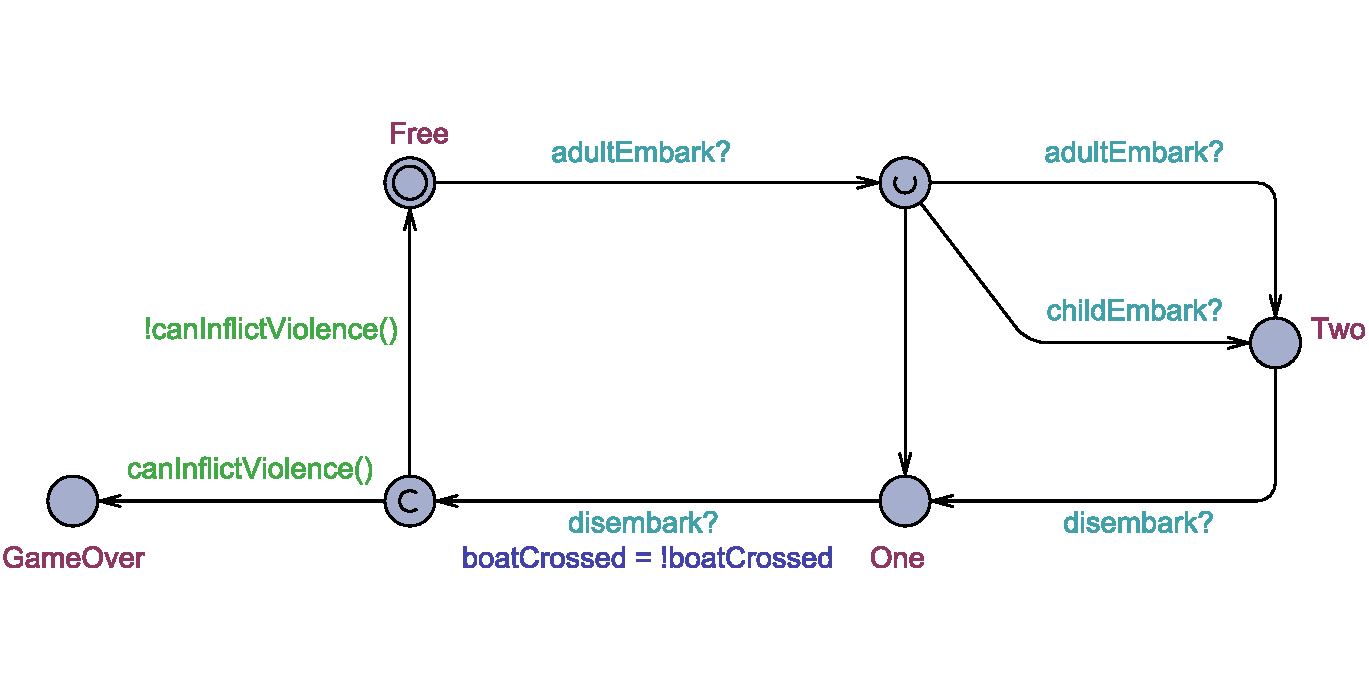
\includegraphics[width=\linewidth]{Boat.pdf}
\caption{Crossing the river}
\end{figure}

\begin{figure}[H]
\centering
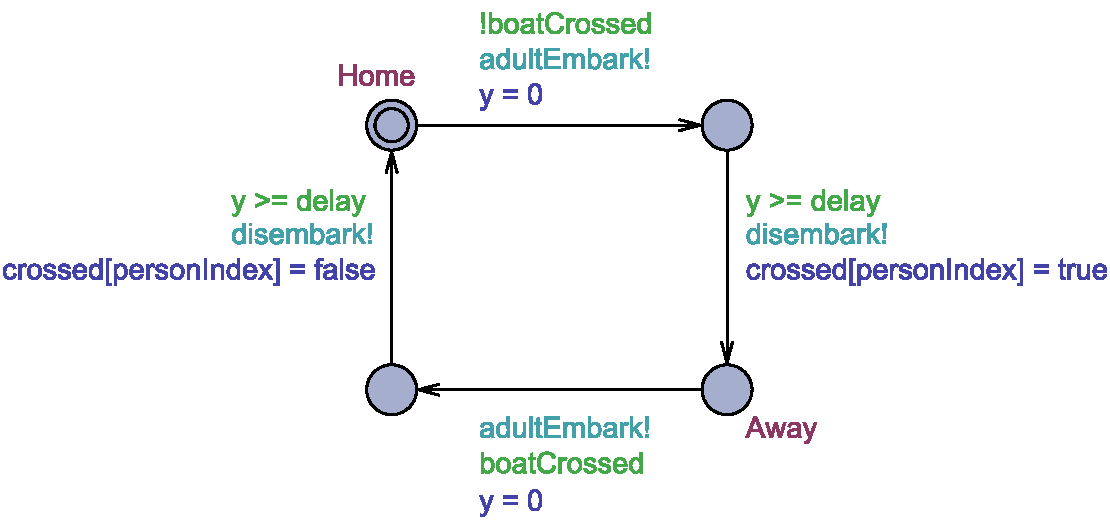
\includegraphics[width=\linewidth]{Adult.pdf}
\caption{Crossing the river}
\end{figure}

\begin{figure}[H]
\centering
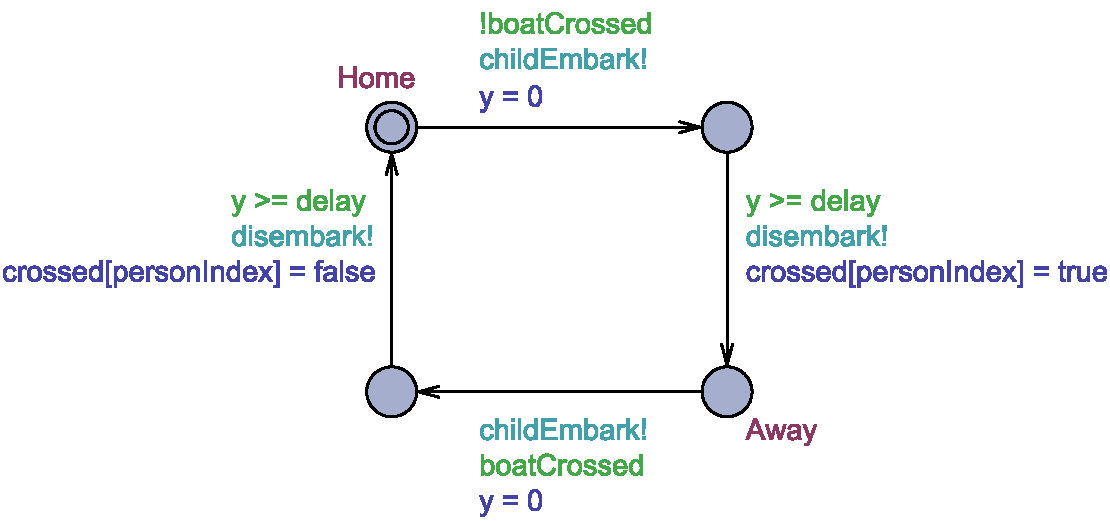
\includegraphics[width=\linewidth]{Child.pdf}
\caption{Crossing the river}
\end{figure}

\begin{lstlisting}[caption={Global declarations}]
// Place global declarations here.

clock time;
bool boatCrossed = false;
chan disembark, childEmbark, adultEmbark;

const int mom = 0;
const int dad = 1;
const int boy1 = 2;
const int boy2 = 3;
const int girl1 = 4;
const int girl2 = 5;
const int police1 = 6;
const int thief1 = 7;

const int boysCount = 3;
const int boys[boysCount] = { boy1, boy2 };

const int girlCount = 3;
const int girls[girlCount] = { girl1, girl2 };

const int policeCount = 2;
const int polices[policeCount] = { police1 };

const int thiefCount = 5;
const int thiefs[thiefCount] = { thief1 };

const int participants = boysCount + girlCount + policeCount + thiefCount + 2; // +2 for parents
bool crossed[participants]; // default array values are false

bool onTheSameSide(int p1, int p2)
{
    return crossed[p1] == crossed[p2];
}

bool boyOnSameSideAs(int personIndex)
{
    // if any boy is on the same side as the person, return true
    for (i : int[0, boysCount-1])
    {
        if (onTheSameSide(personIndex, boys[i]))
        {
            return true;
        }
    }
    return false;
}

bool girlOnSameSideAs(int personIndex)
{
    // if any girl is on the same side as the person, return true
    for (i : int[0, girlCount-1])
    {
        if (onTheSameSide(personIndex, girls[i]))
        {
            return true;
        }
    }
    return false;
}

bool policeOnTheSameSideAs(int personIndex)
{
    // if any dad is on the same side as the person, return true
    for (i : int[0, policeCount-1])
    {
        if (onTheSameSide(personIndex, polices[i]))
        {
            return true;
        }
    }
    return false;
}

bool canMomInflictViolence()
{
    return (boyOnSameSideAs(mom) && crossed[mom] != crossed[dad]);
}

bool canDadInflictViolence()
{
    return (girlOnSameSideAs(dad) && crossed[dad] != crossed[mom]);
}

bool canThiefInflictViolence()
{
    for (i : int [0, thiefCount-1])
    {
        int thiefIndex = thiefs[i];
        if (!policeOnTheSameSideAs(thiefIndex) && (crossed[thiefIndex] == crossed[mom] || crossed[thiefIndex] == crossed[dad] ||
           boyOnSameSideAs(thiefIndex) || girlOnSameSideAs(thiefIndex)))
        {
            return true;
        }
    }
    return false;
}

bool canInflictViolence()
{
    return canMomInflictViolence() || canDadInflictViolence() || canThiefInflictViolence();
}

bool allCrossed()
{
    for (i : int[0, participants-1])
    {
        if (!crossed[i])
        {
            return false;
        }
    }
    return true;
}
\end{lstlisting}

In order to create instances of \lstinline|Adult|s and \lstinline|Childs| we need to give them a unique index. The index is passed to the processes when they are declared as well as a constant amount of time they take to cross the river \lstinline|Boy1 = Child(boy1, fast)|.

All the unique indices are declared at lines 7-14 and the indices belonging to boys, girls, policemen, and thieves are put into their respective arrays at lines 16-27. So in order to add a boy/girl/policeman/thief to the system we only need to create a unique index $i$ such that $i \in [0 ... |participants|-1]$ which will correspond to their index in the \lstinline|crossed[ ]| array, then add the boy/girl/policeman/thief to their respective array, and remember to increment the count of that type of person. After that we of course also need to create the process for that person and them pass them their index.

If UPPAAL allowed us to get the size of an array passed as a parameter to a function then we could cut our code in half. We would not need to keep count of how many boys/girls/policemn/thieves we had, and we would only need one function to check whether a given person is on the same side as any type of person.

The \lstinline|allCrossed()| function checks whether all people in the game has crossed the river. This function is only used to query whether everyone crossed the river.

\section*{Conclusion}

With our UPPAAL model we can verify that it is possible to have everyone cross the river without anyone getting violent on each other. Trying to add just one boy/girl/thief leads to the game being unsolvable. If we add a policeman so we have two, then we can have as many boys/girls/thieves as we like.

We added time to our model. The childs/adults are then instantiated with the time they take to cross the river. Then with our global time variable, UPPAAL could see tell us the shortest time it takes for everyone to cross the river.

\end{document}